\section{Chromium dimer}

Chromium dimmer has been a challenging problem in quantum chemistry, because large active space is needed to simulate its potential energy curve correct. At the same time, dynamic correlation is also required for a qualitative potential energy curve. \cite{andersson_cr2_1994,roos_multiconfigurational_1995,roos_multiconfigurational_1996,roos_ground_2003,angeli_third-order_2006,muller_large-scale_2009,kurashige_second-order_2011,sharma_multireference_2015}
%Perturbation theory is relatively cheap among methods for dynamic correlation, such as multi-reference couple cluster, multi-reference configuration interaction. It is widely used in the chromium dimmer calculations. 

The CAS(12e,12o), derived from the 3d and 4s atomic orbitals, was widely employed for chrmium dimer calculations.\cite{andersson_cr2_1994,roos_multiconfigurational_1995,roos_multiconfigurational_1996,angeli_third-order_2006,muller_large-scale_2009,sharma_multireference_2015} Both CASPT2\cite{andersson_cr2_1994,roos_multiconfigurational_1995,roos_multiconfigurational_1996} and NEVPT2\cite{angeli_n-electron_2001} based CASSCF(12e,12o) reference function overestimate the dissociation energy of the 3d-3d bond, especially when large basis sets, e.g. g-, h-, or even i- type function, were used.\cite{celani_cipt2_2004,angeli_third-order_2006} And the results from CASPT2(12e,12o) are heavily sensitive to the choice of the zero-order Hamiltonian.\cite{celani_cipt2_2004,ruiperez_complete_2011}
According to NEVPT3 study,\cite{angeli_third-order_2006} the common CAS(12e,12o) wave function is not a good starting reference for the perturbation theory, because the third-order perturbation results in an large fluctuation and an unreasonably curve. DMRG-CASPT2 calculation with a CAS(12e,28o), derived from 3d, 4s, 4p, 4d atomic orbitals, gave potential energy curves close to the experimental one. However, different zero-order Hamiltonians, due to different level shifts in CASPT2, gave quantitatively different results. The difference of $D_e$ with different level shifts was about 0.2eV.
\cite{kurashige_second-order_2011}
DMRG-NEVPT2 is free of intruder state and there is no need add ``level shift'' to change zero-order Hamiltonian. It should be feasible to discribe chromium dimer potential energy curve.

\begin{figure}\label{fig:12o_nevpt2}
  \includegraphics[width=8cm,height=6cm]{application/12o-nevpt2.eps}
  \caption{NEVPT2(12e,12o) potential energy curve with a suite cc-pvxz basis set (x=t,q,5)}
  {\footnotesize The Energy is relative to the isolated atoms. }
\end{figure}

A suite of cc-pvxz (x = t,q,5) basis sets was used in our calculations. No basis set superposition error (BSSE) corrections were applied in the calculations because the BSSE was regarded as small for the large basis sets including h or i-type functions. Isolated atoms were used as energy reference, which was consistent with extremely long ($30\mbox{\AA}$) dimer.
%The symmetry of an isolated atom was set as $C_{\infty v}$, while the dimer's symmetry is set as $D_{\infty h}$. Otherwise, the isolated atom's CAS(6e,9o) will be not consistent with the CAS for the dimer.

For the NEVPT2(12e,12o) potential energy curve of Cr$_2$ in \ref{fig:12o_nevpt2}, larger basis set gives a deeper and, sometimes, worse, curve. It is agree with previous studies with atomic natural orbital (ANO) basis sets.
%Our DMRG-NEVPT2 calculations used the cc-pvxz (x = t,q,5) basis sets. 
Then the (12e,12o) CAS was extended by adding \{$\sigma_g,\sigma_u,\pi_g,\pi_u,\pi'_g,\pi'_u$\} orbitals, dominant compoents of which are $4p$ and $4d$ orbitals (after orbital optimization, mainly $4d$ orbitals), forming a (12e,18o) CAS. Due to exponential computation of FCI, DMRG becomes neccesary.
Before DMRG-NEVPT2 calculation, orbitals were optmized with DMRG-SCF with $M=1000$, through Pyscf and Block. There was no frozen core in the orbital optimization. Then reference MPS was optimized with M=4000 and was then compressed into a MPS with M=1000 through ``reverse schedule'', with the optimized CAS. To check whether $M$ is big enough, the potential energy curve with ccpv5z basis was also calculated with M=1500. The difference between curving with M=1000 and that with M=1500 is ignorable.


\begin{figure}
  %\includegraphics[width=8cm,height=6cm]{application/M1000-1500.eps}
\includegraphics[width=0.6\textwidth]{application/M1000-1500.eps}
  \caption{DMRG-NEVPT2(12e,18o) results with different bond dimension}

\end{figure}

\begin{figure}\label{fig:5qt_fitting}
  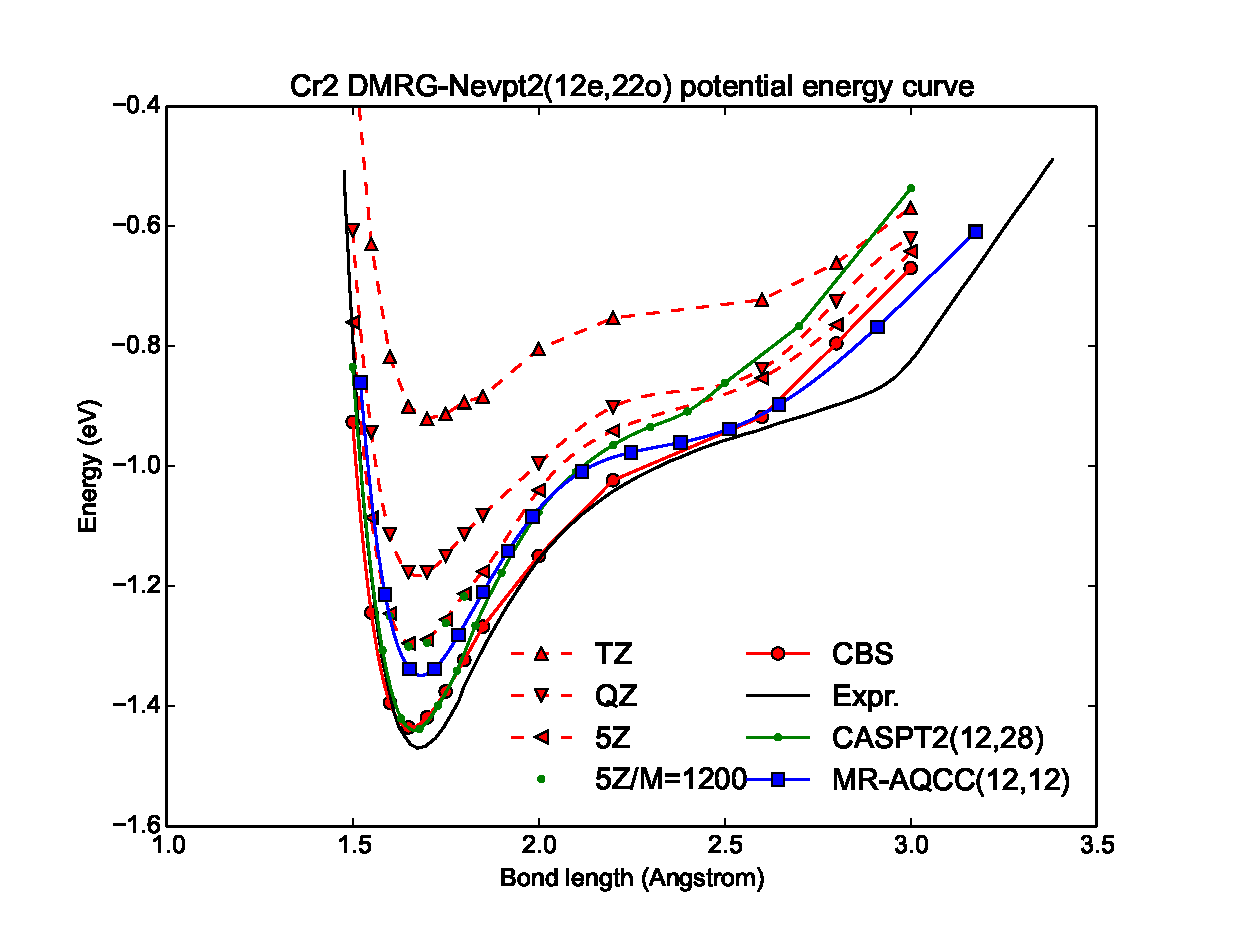
\includegraphics[width=8cm,height=6cm]{application/5qt-fitting.eps}
  \caption{DMRG-NEVPT2(12e,18o) potential energy curve with a suite cc-pvxz basis set (x=t,q,5) and CBS limit}
  %\caption{NEVPT2(12e,12o) and DMRG-NEVPT2(12e,18o) potential energy curve with a suite cc-pvxz basis set (x=t,q,5) and CBS limit}
\end{figure}

Figure \ref{fig:5qt_fitting} shows the potential energy curve with a suite of cc-pvxz (x=t,q,5) basis set and complete basis set (CBS) limit. A larger basis set still gives a deeper and better (not like CAS(12e,12o) result) curve. 

%The calcualted $D_e$ is 1.491eV, very close to the experimental value 1.47eV \cite{casey_negative_1993}. However, the calculated bond length is shorter than experimental value. 

\begin{table}
  \begin{tabular}{cccc}
  \toprule
      & $D_e(eV)$ & $R_0($\AA$)$ & $\omega_e$ \\
  \midrule
    ccpv-$x$z CAS(12e,18o) & 1.491 & 1.632 & 415 \\ 
  \midrule
  experiment & 1.47(5) & 1.679 & 480.6(5) \\
  \bottomrule
  \end{tabular}
\end{table}


%FIXME
Need logical reasons here.
In the calculation discribed above, the relativistic effect was not included. And cc-pv$x$z basis set might not be able to describe core-valence correlation well.
The calculated potential energy curve was already quantitatively correct, compared to expermiental one. However, there is definitely not enough evindence to say that relativeistic effect is not important or that cc-pv$x$z basis is enough for core-valence correaltions.
%FIXME
We used cc-pwcv$x$z-dk basis set and x2c Hamiltonian to get better accuracy.

At the same time, the $4d$ orbital were not fully included in the active space, only $d_{z^2}$,$d_{xz}$,$d_{yz}$. $\delta$ bonds formed by $d_{xy}$ and $d_{x^2-y^2}$ were not included, because their orbital energies in mean-field and CASSCF (CAS(12e,12o)) calculations were higher than those of $4d$ $\sigma$ and $\pi$ orbitals. Including them in the active space would give a better result. However, the computations increased a lot. We had to decrease the bond dimension to 500 in DMRG-NEVPT2 calculation.